\documentclass{article}
\usepackage{geometry}
\usepackage{graphicx}
\graphicspath{ {./} }

\geometry{margin=0.75in}


\begin{document}

\title{Riešenie 4. úlohy kategórie B}
\author{Jozef Komáromy}

\maketitle

\section{Podúloha A}

\begin{figure}[h]
  \centering
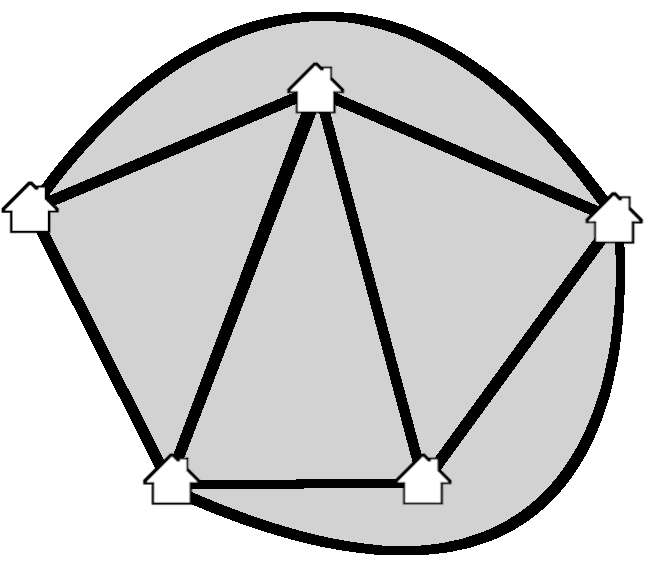
\includegraphics{A}
\end{figure}

\section{Podúloha B}



\section{Podúloha C}

Vzťah medzi celkovým počtom ciest \(n\) a počtom častí na ktoré by bola lúka rozdelená \(p\) by bol nasledovný: \(p = 2 + 2 * (n - 3)\). Je to tak pretože uzavretý obvod kruhu delí lúku na 2 časti a každá nasledovne pridaná cesta oddelí 1 ďalšiu časť lúky.

\section{Podúloha D}



\section{Podúloha E}

Najviac sa dá postaviť \(n + 2 * (n - 3)\) ciest. Prvých \(n\) ciest bude tvoriť uzavrétý obvod kruhu. Ďalších \(n - 3\) ciest bude viesť z ľubovolného domu do domov s ktorými nie je spojený, tieto cesty sa budú nachádzať vo vnútri pôvodného kruhu domov. Posledných \(n - 3\) ciest bude viesť z iného ľubovolného domu do domov s ktorými nie je spojený, tieto cesty sa budú nachádzať na vonkajšej strane kruhu.

\end{document}
